\documentclass[12pt, twoside]{book}
\usepackage[a4paper,top=2.5cm,bottom=2.5cm,left=3.5cm,right=2cm]{geometry}
\usepackage[utf8]{inputenc}
\usepackage[T1]{fontenc}
\usepackage{graphicx}
\usepackage{url}
\usepackage{babel}
\usepackage{tikz}
\usetikzlibrary{positioning}
\usepackage[hidelinks,breaklinks]{hyperref}
\linespread{1.25} % hodnota 1.25 by mala zodpovedat 1.5 riadkovaniu

% -------------------
% --- Definicia zakladnych pojmov
% --- Vyplnte podla vasho zadania
% -------------------
\def\mfrok{2020}
\def\mfnazov{Material picker: Material recognition in images using deep learning}
\def\mftyp{Bachelor Thesis}
\def\mfautor{Filip Jurčák}
\def\mfskolitel{prof. RNDr. Roman Ďurikovič, PhD.}

%ak mate konzultanta, odkomentujte aj jeho meno na titulnom liste
\def\mfkonzultant{Mgr. Petr Vévoda}  

\def\mfmiesto{Bratislava, \mfrok}

\def\mfodbor{Computer Science}
\def\program{Computer Science}

% Ak je školiteľ z FMFI, uvádzate katedru školiteľa, zrejme by mala byť aj na zadaní z AIS2
% Ak máte externého školiteľa, uvádzajte Katedru informatiky 
\def\mfpracovisko{ FMFI.KI - Department of Computer Science }

\begin{document}     
\frontmatter


% -------------------
% --- Obalka ------
% -------------------
\thispagestyle{empty}

\begin{center}
  \sc\large
  Comenius University in Bratislava\\
  Faculty of Mathematics, Physics and Informatics

\vfill

{\LARGE\mfnazov}\\
\mftyp
\end{center}

\vfill

{\sc\large 
\noindent \mfrok\\
\mfautor
}

\cleardoublepage
% --- koniec obalky ----

% -------------------
% --- Titulný list
% -------------------

\thispagestyle{empty}
\noindent

\begin{center}
\sc  
\large
  Comenius University in Bratislava\\
  Faculty of Mathematics, Physics and Informatics

\vfill

{\LARGE\mfnazov}\\
\mftyp
\end{center}

\vfill

\noindent
\begin{tabular}{ll}
Study Programme: & \program \\
Field of Study: & \mfodbor \\
Department: & \mfpracovisko \\
Supervisor: & \mfskolitel \\
Consultant: & \mfkonzultant \\
\end{tabular}

\vfill


\noindent \mfmiesto\\
\mfautor

\cleardoublepage
% --- Koniec titulnej strany


% -------------------
% --- Zadanie z AIS
% -------------------
% v tlačenej verzii s podpismi zainteresovaných osôb.
% v elektronickej verzii sa zverejňuje zadanie bez podpisov
% v pracach v naglictine anglicke aj slovenske zadanie

\newpage 
\thispagestyle{empty}
\hspace{-2cm}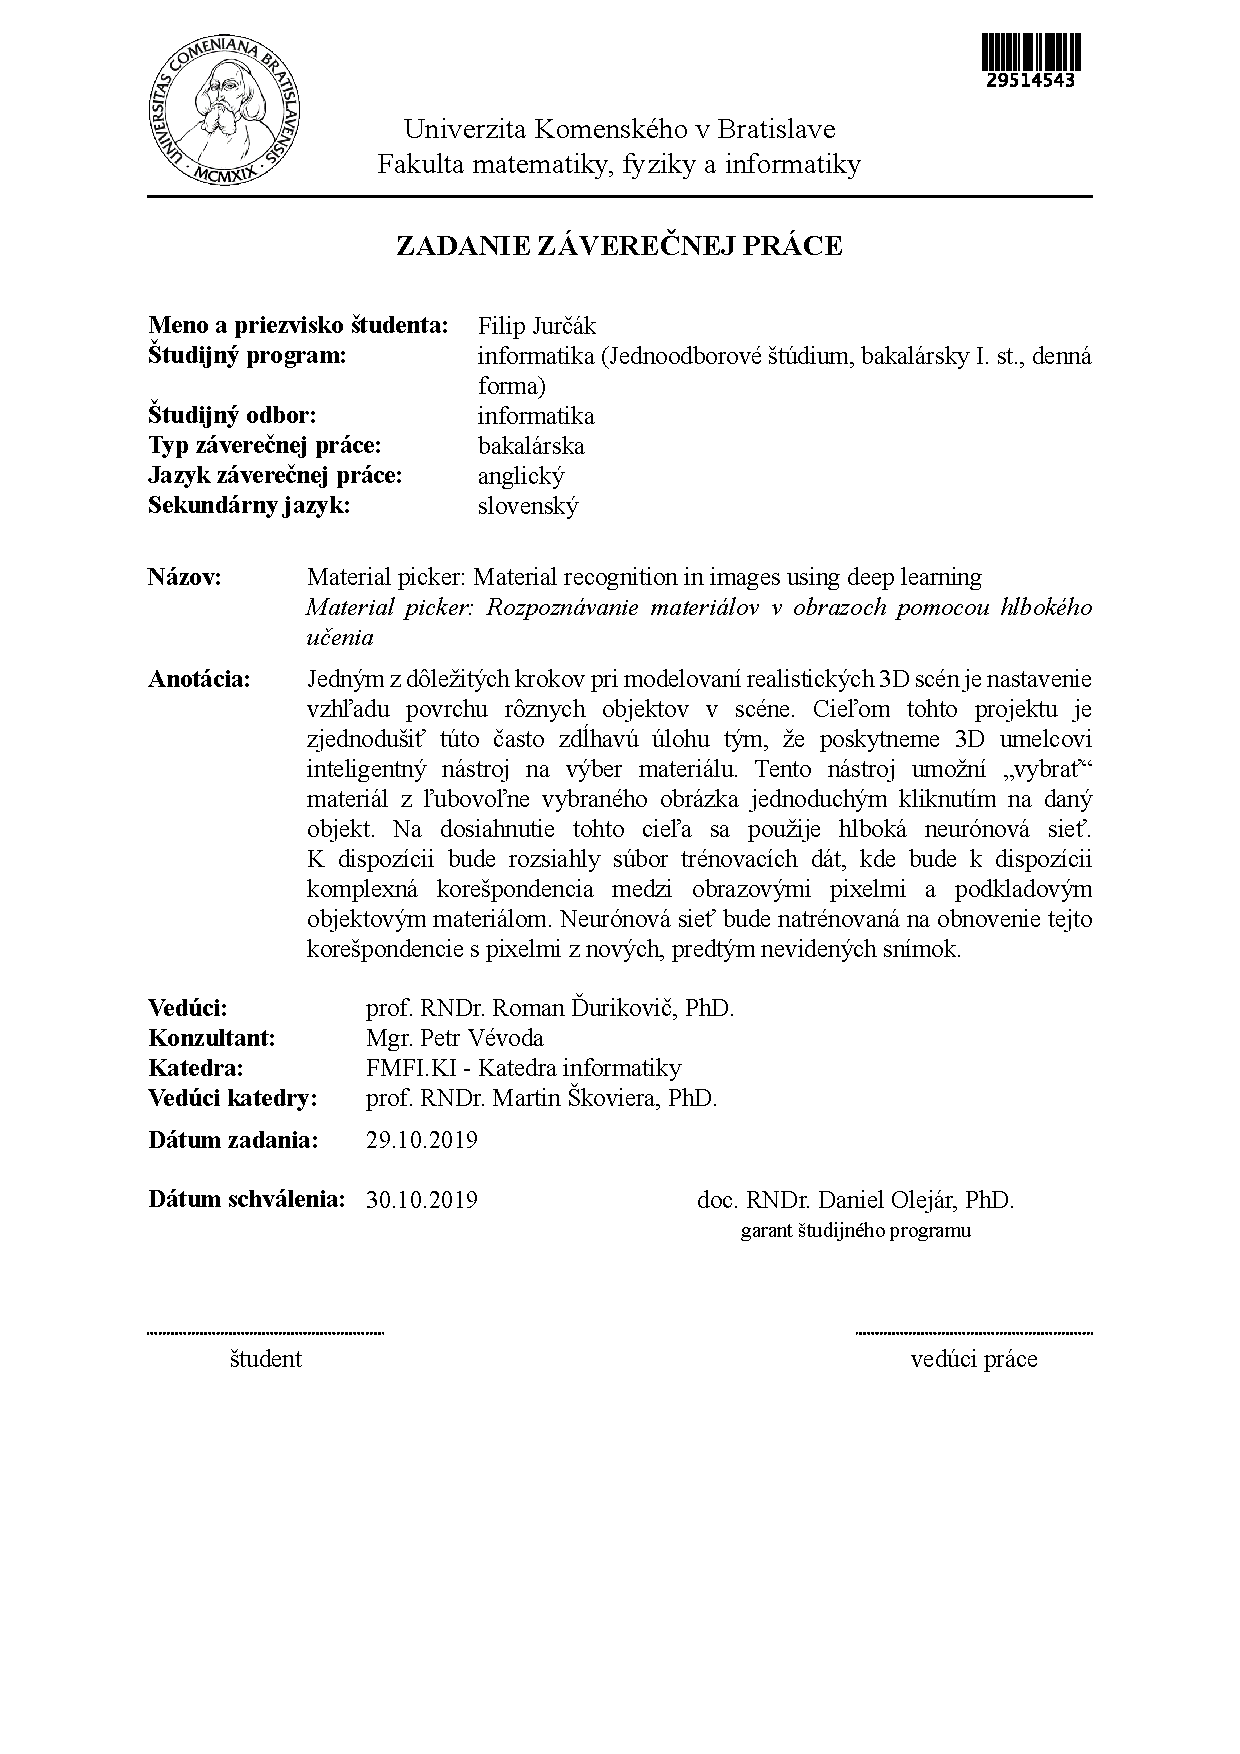
\includegraphics[width=1.1\textwidth]{praca/images/zadanie-jurcak-sk.pdf}

\hspace{-2cm}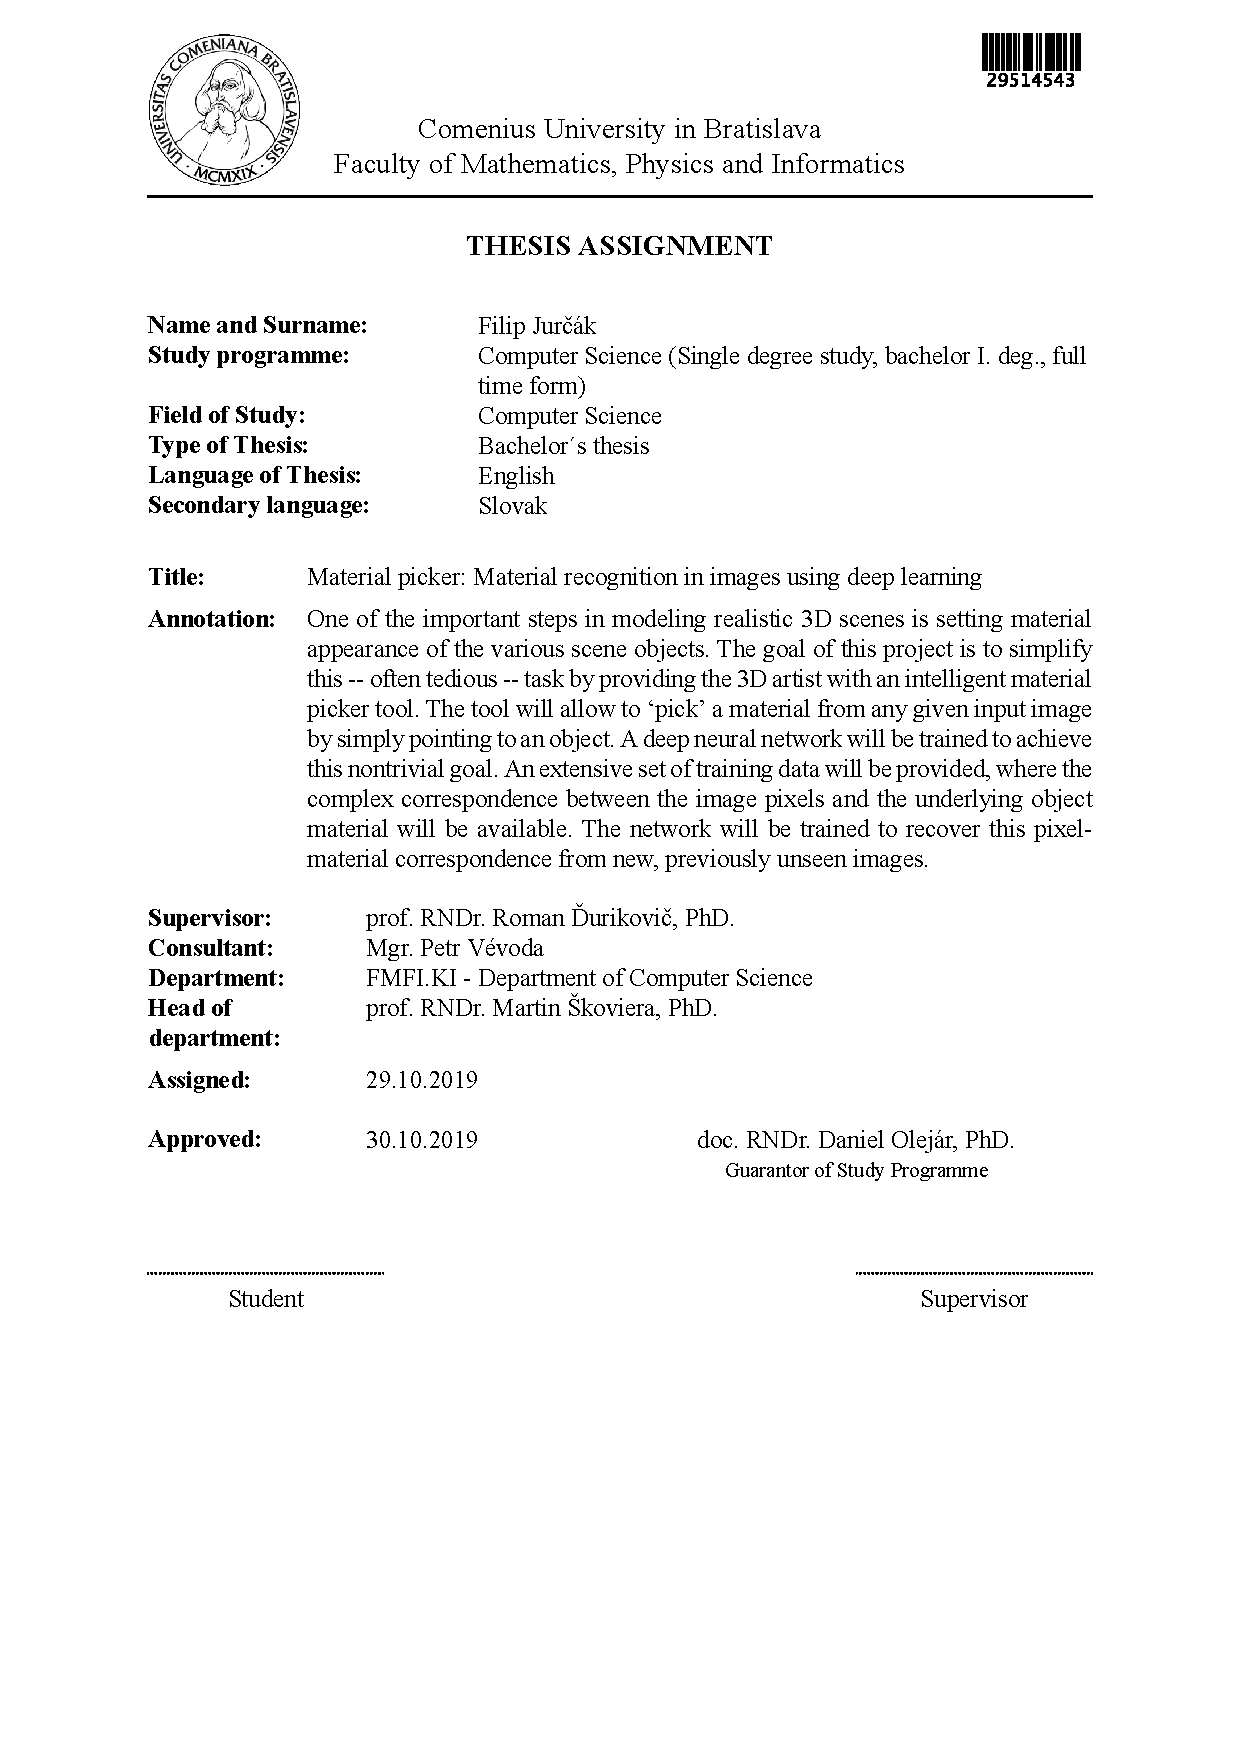
\includegraphics[width=1.1\textwidth]{praca/images/zadanie-jurcak-en.pdf}

% --- Koniec zadania

\frontmatter

% -------------------
%   Poďakovanie - nepovinné
% -------------------
\setcounter{page}{3}
\newpage 
~

\vfill
% {\bf Acknowledgments:} Tu môžete poďakovať školiteľovi, prípadne
% ďalším osobám, ktoré vám s prácou nejako pomohli, poradili,
% poskytli dáta a podobne.

% --- Koniec poďakovania

% -------------------
%   Abstrakt - Slovensky
% -------------------
\newpage 
\section*{Abstrakt}


Jedneho dna tu bude pekny abstrakt. Dnes nie je ten den.

\paragraph*{Kľúčové slová:}
% --- Koniec Abstrakt - Slovensky


% -------------------
% --- Abstrakt - Anglicky 
% -------------------
\newpage 
\section*{Abstract}

Abstract in the English language (translation of the abstract in the
Slovak language).


\paragraph*{Keywords:} 

% --- Koniec Abstrakt - Anglicky

% -------------------
% --- Predhovor - v informatike sa zvacsa nepouziva
% -------------------
%\newpage 
%\thispagestyle{empty}
%
%\huge{Predhovor}
%\normalsize
%\newline
%Predhovor je všeobecná informácia o práci, obsahuje hlavnú charakteristiku práce 
%a okolnosti jej vzniku. Autor zdôvodní výber témy, stručne informuje o cieľoch 
%a význame práce, spomenie domáci a zahraničný kontext, komu je práca určená, 
%použité metódy, stav poznania; autor stručne charakterizuje svoj prístup a svoje 
%hľadisko. 
%
% --- Koniec Predhovor


% -------------------
% --- Obsah
% -------------------

\newpage 

\tableofcontents

% ---  Koniec Obsahu

% -------------------
% --- Zoznamy tabuliek, obrázkov - nepovinne
% -------------------

\newpage 

\listoffigures
\listoftables

% ---  Koniec Zoznamov

\mainmatter


\input introduction.tex 

\input problem_statement.tex

\input prior_work.tex

\input our_approach.tex

\input dataset.tex

\input implementation.tex

\input results.tex

\input conclusion.tex

% -------------------
% --- Bibliografia
% -------------------


\newpage	

\backmatter

\thispagestyle{empty}
\nocite{*}
\clearpage

\bibliographystyle{plain}
\bibliography{literature}

%---koniec Referencii

% -------------------
%--- Prilohy---
% -------------------

%Nepovinná časť prílohy obsahuje materiály, ktoré neboli zaradené priamo  do textu. Každá príloha sa začína na novej strane.
%Zoznam príloh je súčasťou obsahu.
%
%\input appendixA.tex

%\input appendixB.tex

\end{document}






